\chapter{系统设计与实现}

本章设计并实现了一个具有交互性和用户友好性的基于知识图谱和大语言模型智能体机制的API编排和调用系统。该系统集成了不同模型的调用接口,以及知识图谱查询的功能。该系统提供了一个使用门槛低、用户友好的界面,允许用户通过自然语言的方式与该系统进行交互和提问,系统会根据用户的需求编排并调用所需的API,并进行回答。

% 难点:

% 界面设计:友好交互、展示图谱部分、添加api部分

% 前后端框架选什么

% 前:streamlit 后:fastapi

% 模型管理(不同模型,超参数,上下线) 如何交互 容错 restapi格式 如何加速

% 数据管理 Neo4j qdrant 用户数据 记忆数据

\section{系统需求分析}

\indent 我们采用面向对象的需求分析方法,绘制了如图~\ref{fig:usecase}所示的系统用例图。

\begin{figure}[H]
  \vspace{1em}
  \centering
  \setlength{\abovecaptionskip}{10pt} % 控制图片和caption之间的距离
  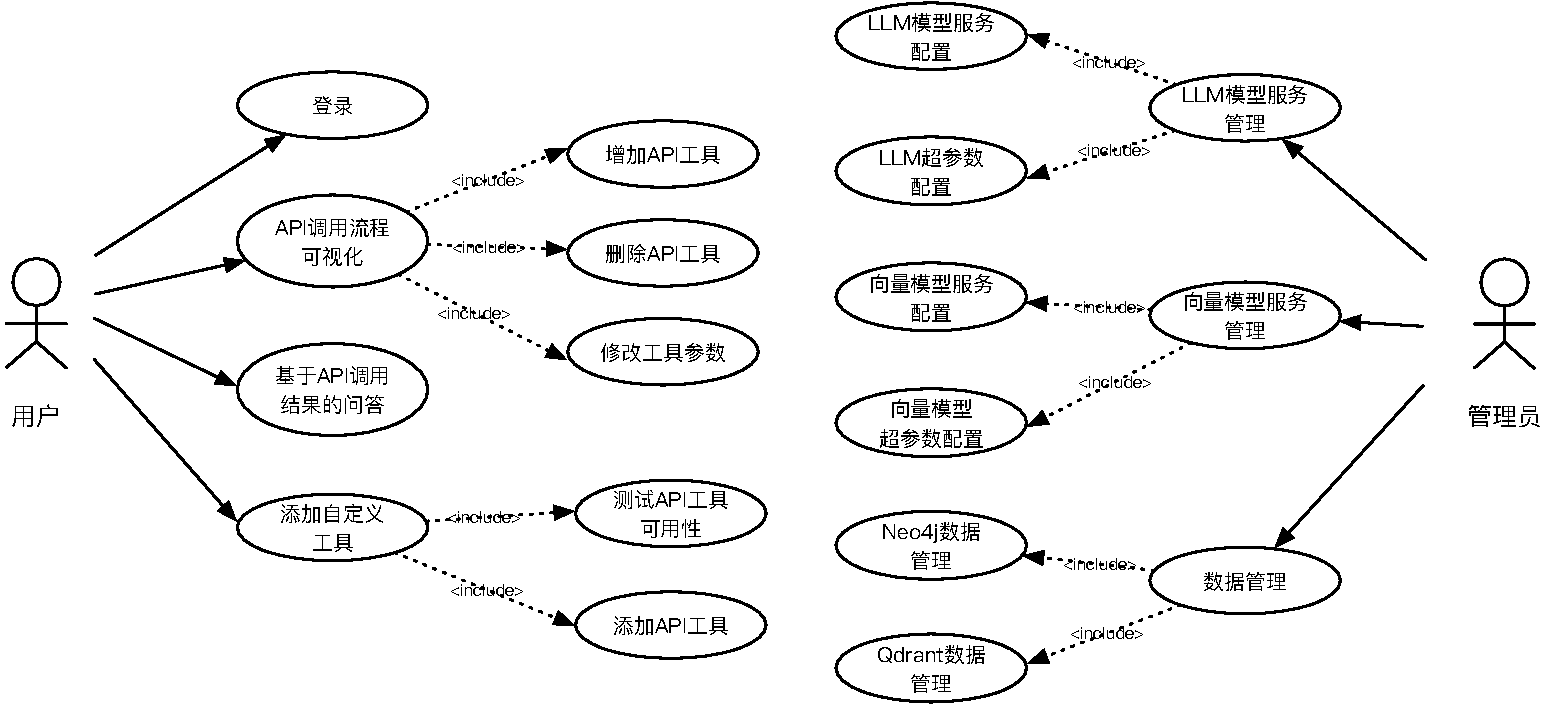
\includegraphics[height=6cm]{../assets/ch5-用例图.pdf}
  \bicaption{系统用例图}{System Usecase Diagram}
  \label{fig:usecase}
\end{figure}

我们采用面向对象的需求分析方法,绘制了系统的用例图。在该用例图中,我们定义了两种主要角色:系统用户和管理人员。系统用户包含普通用户和开发者,而管理人员则具有更高权限的管理功能。这样的角色划分帮助系统满足不同用户的需求,支持工具调用、数据管理、模型管理等任务。根据需求分析,系统应具备以下核心功能模块:

1.	用户与权限管理:系统应提供用户注册、登录、身份验证和权限分配功能。系统用户可根据权限访问相应模块,而管理人员具有配置用户权限的能力,以保障系统安全性和合理性。

2.	API调用流程管理与问答支持:系统支持用户通过可视化界面查看并编辑API调用流程,并能基于调用结果进行问答。API调用流程管理模块可展示调用步骤、输入输出等信息,用户可根据需要进行简单调整。问答模块则负责对编排好的工具流程进行调用和解析,生成总结性描述或回答用户问题。

3.	自定义工具与工具库管理:系统支持用户根据需求添加自定义工具,丰富工具库的扩展性。用户通过填写工具的配置信息并测试后,系统将自动集成到工具库,供用户选择和调用。同时,工具库还提供常用工具模板,方便用户浏览和直接调用。

4.	模型服务管理:系统为管理人员提供大语言模型和向量模型服务的管理功能。该模块支持模型的配置、更新和监控,以满足多种任务需求并优化系统性能。管理人员可以根据需要对模型进行更新,以确保系统提供高效的模型服务。

5. 数据库管理:系统应提供高效的图数据库和向量数据库管理功能,以支持管理员对不同类型的数据进行配置和管理。对于图数据库管理,平台应支持Neo4j等图数据库的配置,允许管理员查看数据库状态、管理数据结构和优化查询性能,以确保关系数据的高效存储和检索。对于向量数据库管理,平台应支持Qdrant等向量数据库的配置,允许管理员调整存储策略和搜索参数,以优化向量数据的存储和检索性能。系统支持大规模向量数据的导入、分片配置和索引更新,确保能够高效完成相似度计算,满足推荐系统和语义搜索等场景的需求。

\section{交互方案设计}

图~\ref{fig:system}为该系统的交互设计图。

\begin{figure}[H]
    \vspace{1em}
    \centering
    \setlength{\abovecaptionskip}{10pt} % 控制图片和caption之间的距离
    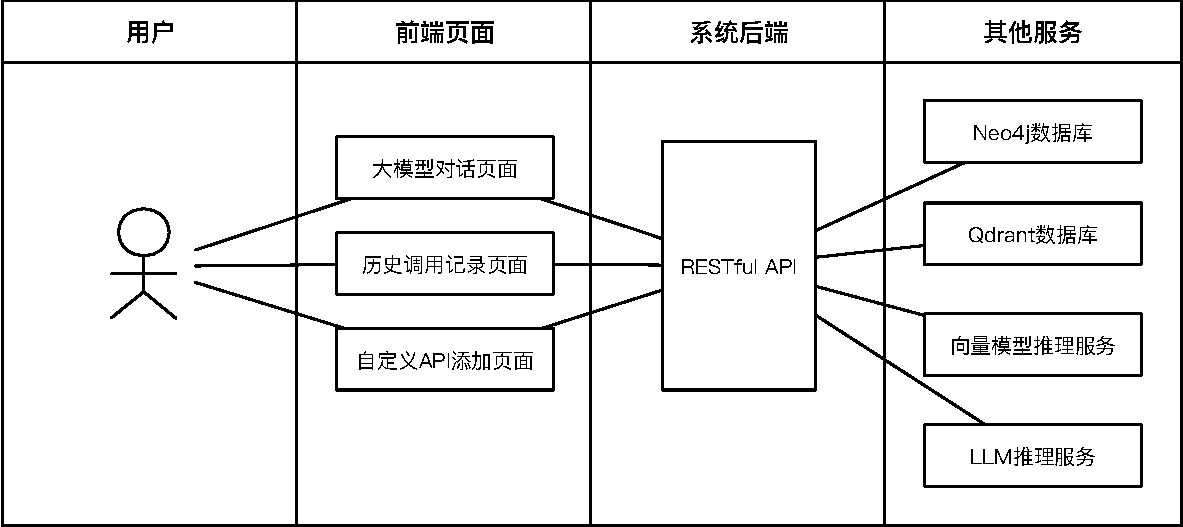
\includegraphics[height=5cm]{../assets/ch5-交互设计图.pdf}
    \bicaption{系统交互图}{System Interaction Diagram}
    \label{fig:interaction}
  \end{figure}

本系统主要有以下三个部分,前端交互界面、系统后端和其他服务模块,集成了不同模型的调用接口以及知识图谱查询功能,为用户提供了低门槛、用户友好的界面,支持用户通过自然语言的方式进行交互和提问。整体交互流程如图6.2所示:

	1.	前端页面:前端页面为用户提供了交互界面,支持大模型对话、历史调用记录以及自定义API工具添加等功能。用户可以通过这些页面与系统进行自然语言交互,例如通过对话界面向大模型提问、查看历史调用模板获取API使用信息,或在自定义页面添加新的API工具以扩展系统功能。
	2.	系统后端:系统后端作为核心控制层,通过RESTful API接口将前端用户请求传递至其他服务模块,并负责业务逻辑的处理。后端系统不仅管理用户请求的权限和数据存储,还充当API编排的核心,确保前端请求的安全性和规范性。在与其他服务模块的交互中,后端可以灵活调用图数据库、向量数据库以及模型推理服务,实现对知识图谱的查询和不同模型的协同调用,以满足复杂的查询和推理需求。
	3.	其他服务模块:其他服务模块包括Neo4j图数据库、Qdrant向量数据库、向量模型推理服务和LLM(大语言模型)推理服务。这些模块分别用于存储和查询图数据库、管理和检索向量化数据、支持基于向量相似度的搜索需求,以及提供大语言模型的对话和推理功能。系统后端根据用户需求对这些服务进行编排调用,确保用户问题得到高效而准确的解答。

通过以上三部分的协同工作,系统能够为用户提供全面的API编排调用智能问答、历史调用模板查询和自定义工具配置等服务,满足用户的需求,并提供了易用、易扩展的系统和良好的交互体验。

\section{系统架构设计}

本系统架构分为五个层次:存储层、访问层、功能层、接口层和展示层。以下对各层的功能和组成模块进行详细介绍。

图~\ref{fig:system}为该系统的系统软件架构设计图。

\begin{figure}[H]
    \vspace{1em}
    \centering
    \setlength{\abovecaptionskip}{10pt} % 控制图片和caption之间的距离
    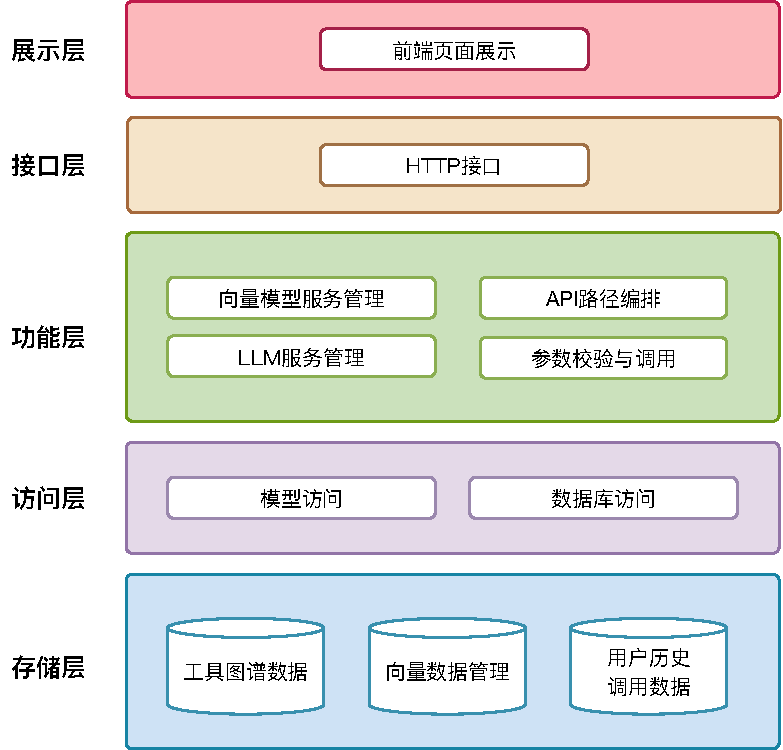
\includegraphics[height=8cm]{../assets/ch5-系统架构图.pdf}
    \bicaption{系统用例图}{System Usecase Diagram}
    \label{fig:system}
  \end{figure}

\subsection{存储层}

存储层负责系统核心数据的存储,包括以下内容:
\begin{itemize}
    \item \textbf{API知识图谱}:用于存储API的知识关联信息,方便后续的关系检索和动态编排。
    \item \textbf{API详细信息的向量存储}:将API的详细信息预先计算并存储在向量数据库中,以便于快速计算相似度。
    \item \textbf{历史调用路径}:记录系统使用过程中产生的调用路径,作为经验数据供后续参考和优化。
\end{itemize}

\subsection{访问层}

访问层负责封装对存储层的访问功能,提供统一的数据访问接口,便于功能层的调用。其主要功能包括:
\begin{itemize}
    \item 访问图数据库和向量数据库的数据,进行知识图谱检索和相似性计算。
    \item 访问和解析JSON格式的文件数据,确保数据在各层之间的顺畅传递。
\end{itemize}

\subsection{功能层}

功能层是系统的核心,实现动态API编排和调用。主要模块包括:

\begin{itemize}
  \item \textbf{任务分解模块}:输入用户的复杂需求,输出为拆解后的固定格式的一组子任务,子任务之间相互独立。
  \item \textbf{长期记忆检索模块}:根据当前任务描述,在历史调用路径中检索相似任务描述和历史调用路径,提供给当前任务的动态API编排模块作为参考。
  \item \textbf{API知识图谱检索模块}:按照不同的检索模式搜索API节点及其关联的邻居节点信息。
  \item \textbf{基于图谱的DFS动态编排算法模块}:在知识图谱上执行深度优先搜索和回溯操作,生成最优的调用路径。
  \item \textbf{API调用模块}:获取目标API的参数信息,并结合用户需求生成API调用的输入参数。使用生成的参数调用API,同时设置自动重试机制,以确保调用的稳定性;若调用失败则进行重试,若多次重试仍失败则返回错误信息。
  \item \textbf{API调用结果总结模块}:将API调用结果转换为自然语言格式,并结合用户的原始需求生成最终的总结性回复。
\end{itemize}

\subsection{接口层}

接口层负责为系统各功能提供访问接口,采用RESTful API的HTTP接口形式:
\begin{itemize}
    \item 系统后端通过RESTful API接口与前端交互,供前端进行数据访问和操作。
    \item 模型服务与平台后端之间也通过HTTP接口进行通信,以确保数据传输的安全性和高效性。
\end{itemize}

\subsection{展示层}

展示层是面向用户的web前端页面,为用户提供直观友好的交互界面。主要页面包括:
\begin{itemize}
    \item \textbf{信息问答页面}:用户可通过自然语言输入需求,系统将自动编排API调用路径并执行,最终以自然语言格式返回结果,模拟多轮对话的交互体验。
    \item \textbf{自定义API添加页面}:用户填写API名称、调用链接、参数类型和描述信息等来添加新API。新API需经过测试验证后方可加入API仓库。
    \item \textbf{API历史调用参考页面}:用户可以查看历史API调用记录,并支持通过选择和配置参数重新使用历史API调用链。
\end{itemize}

\section{模块设计}

图~\ref{fig:module}展示了系统详细的功能层次结构。本系统的详细功能主要包含:用户验证、数据管理、模型服务管理、API工作流编排、API调用问答、自定义API存储。

\begin{figure}[H]
  \vspace{1em}
  \centering
  \setlength{\abovecaptionskip}{10pt} % 控制图片和caption之间的距离
  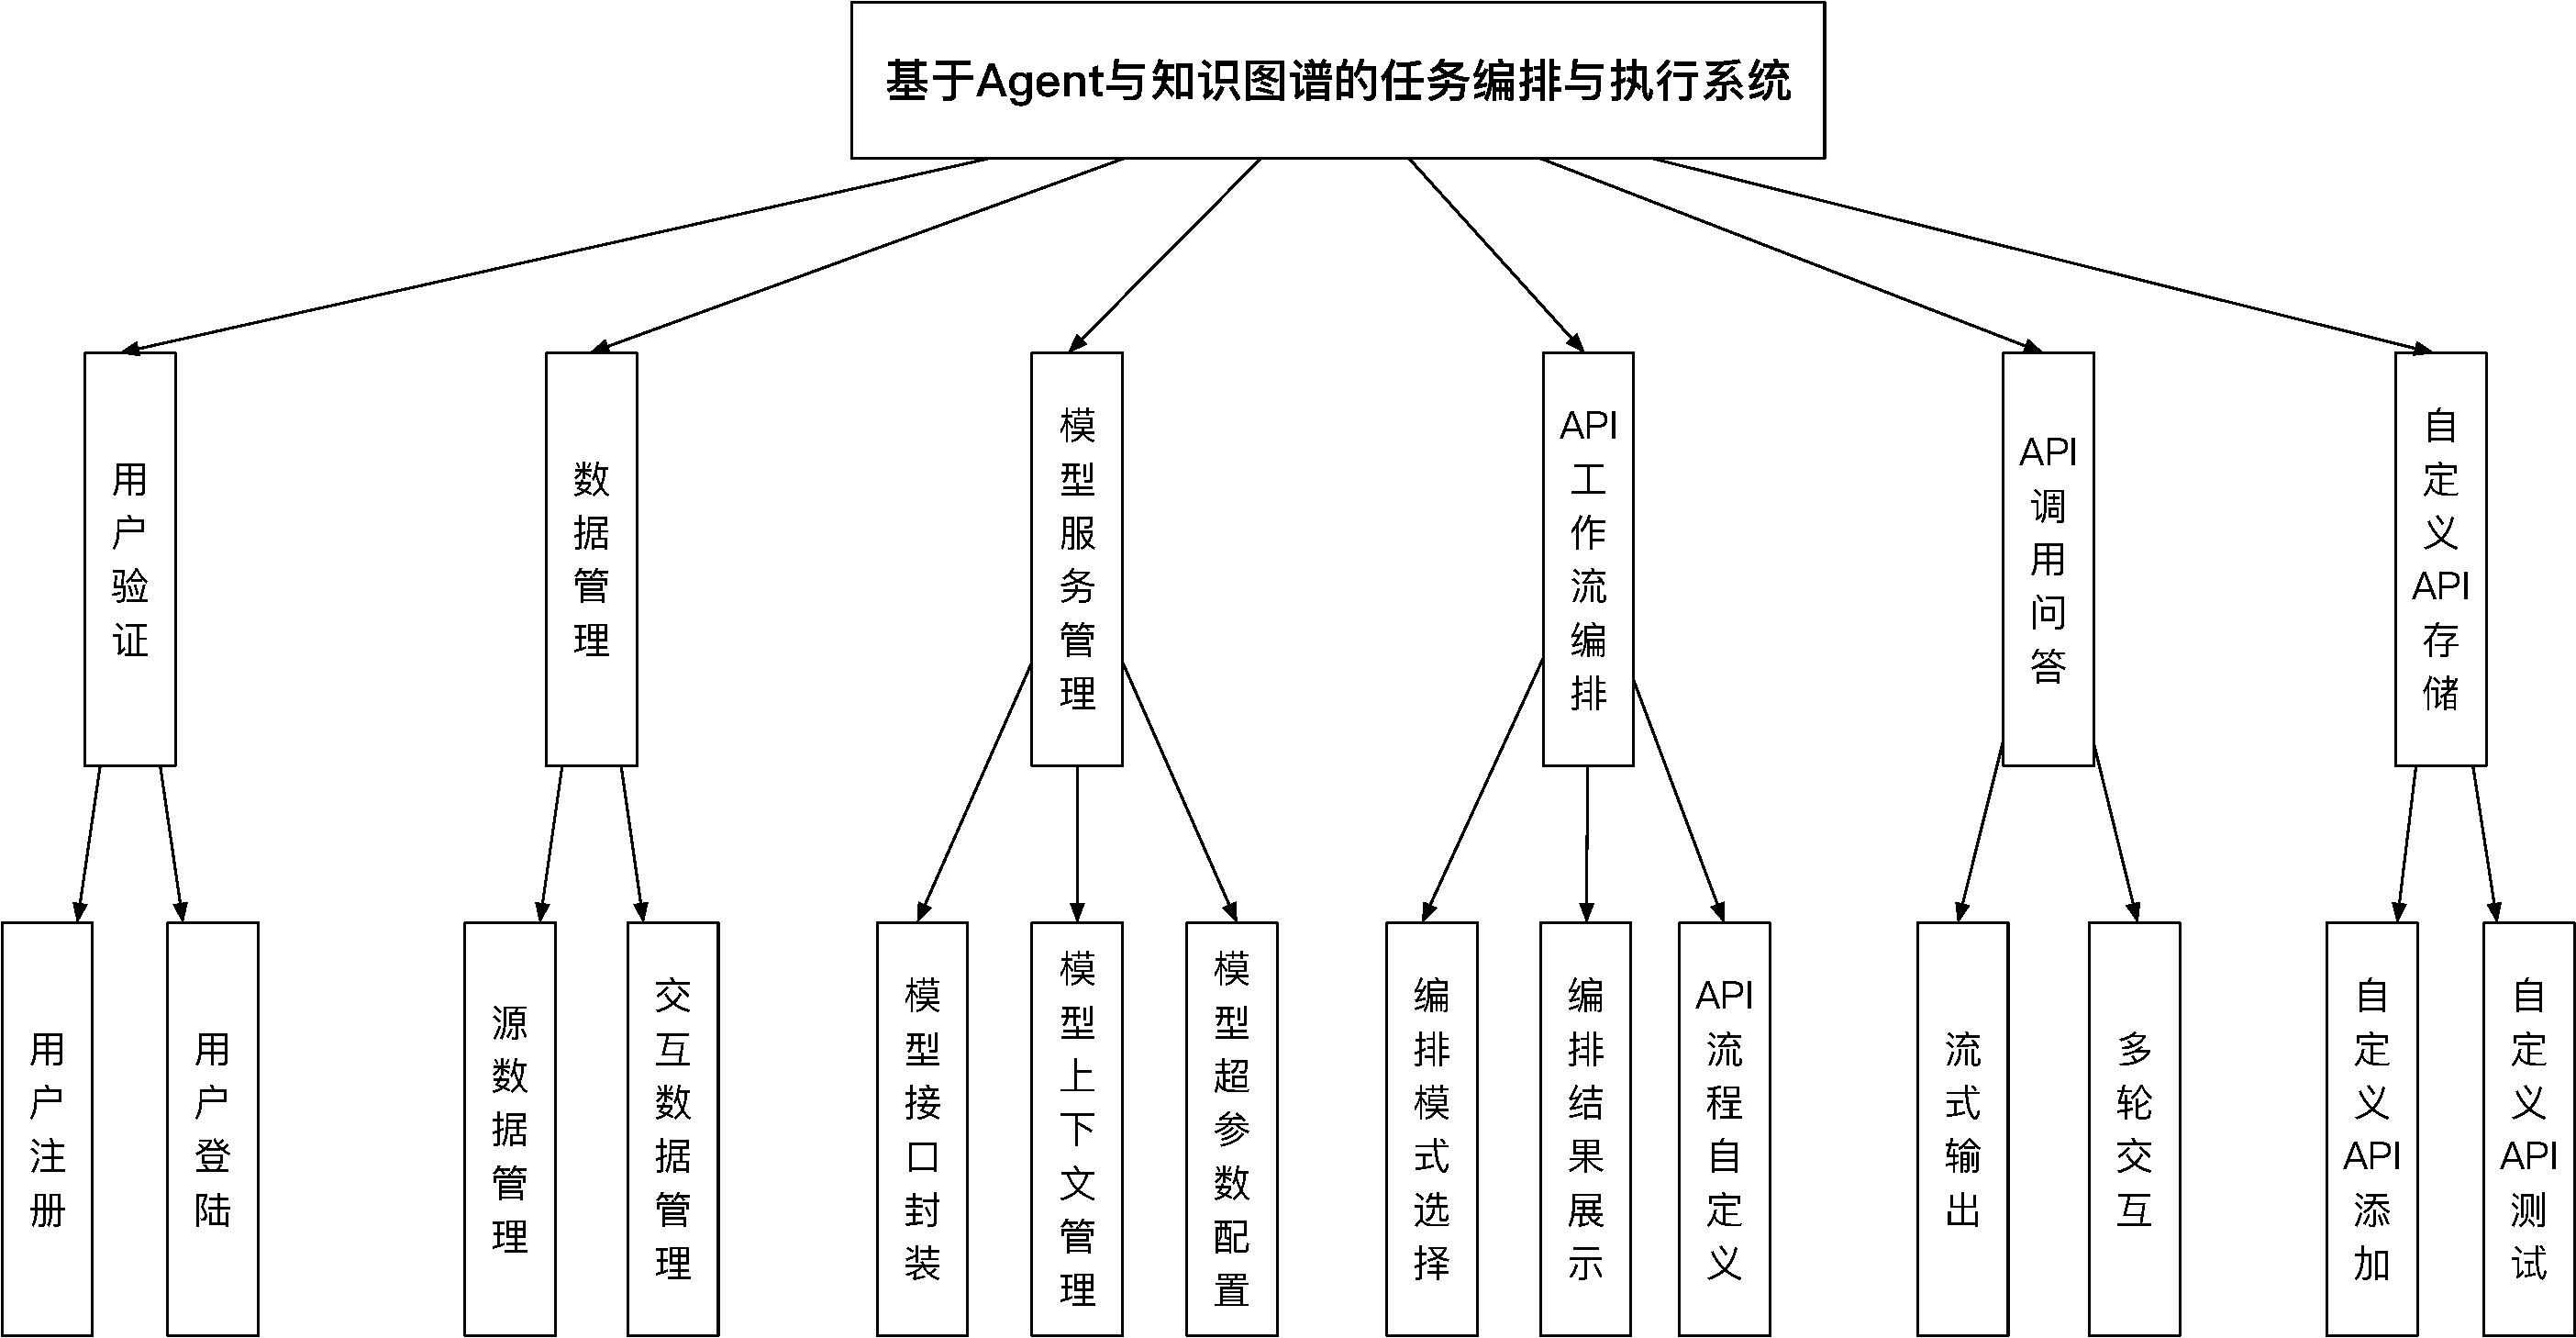
\includegraphics[height=7cm]{../assets/ch5-系统模块图.pdf}
  \bicaption{系统模块图}{System Module Diagram}
  \label{fig:module}
\end{figure}

\subsection{用户验证}
用户验证模块用于实现面向用户的API调用历史记录和模板库构建。该模块包含用户注册和登录功能,允许用户通过注册获得个人账号并登录系统使用。

\subsection{数据管理}
数据管理模块用于管理系统中的各类数据,包括知识图谱数据、API信息向量以及用户交互过程中的历史需求、API编排和调用结果等。主要存储在Neo4j和Qdrant向量数据库中。

\subsection{模型服务管理}
模型服务管理模块包括模型接口封装和模型超参数配置功能。封装不同模型的调用代码为统一接口,对系统其他部分隐藏模型的具体细节。超参数配置则管理模型调用时的参数,如温度系数、最大长度、top\_k、top\_p等。

\subsection{API工作流编排}
API工作流编排模块包含以下三个子模块:
\begin{itemize}
    \item \textbf{编排模式选择}:提供用户可配置的编排选项。
    \item \textbf{编排结果展示}:通过可编辑任务框展示API编排结果,任务框中展示API名称、描述、参数等信息。
    \item \textbf{API流程自定义}:允许用户在生成的API流程基础上,进行增加、删除或修改,支持更灵活的API调用。
\end{itemize}

\subsection{API调用问答}

API调用问答模块通过流式输出和多轮交互,提升用户体验。流式输出模块增强用户等待结果时的体验,多轮交互模块保存上下文中的API调用结果,支持进一步提问。

\subsection{自定义API存储}
自定义API存储模块通过API添加和测试模块,支持用户将自定义API添加到系统中,提高系统扩展性和可用性。

\section{系统实现}

本节将会介绍系统的实现方法。首先是技术选型方面,考虑到与大语言模型、深度学习有关的代码都采用Python编写,我们也采用了Python技术栈。

图\ref{fig:ch6-implementation}为该系统的技术实现图。

\begin{figure}[H]
  \vspace{1em}
  \centering
  \setlength{\abovecaptionskip}{10pt} % 控制图片和caption之间的距离
  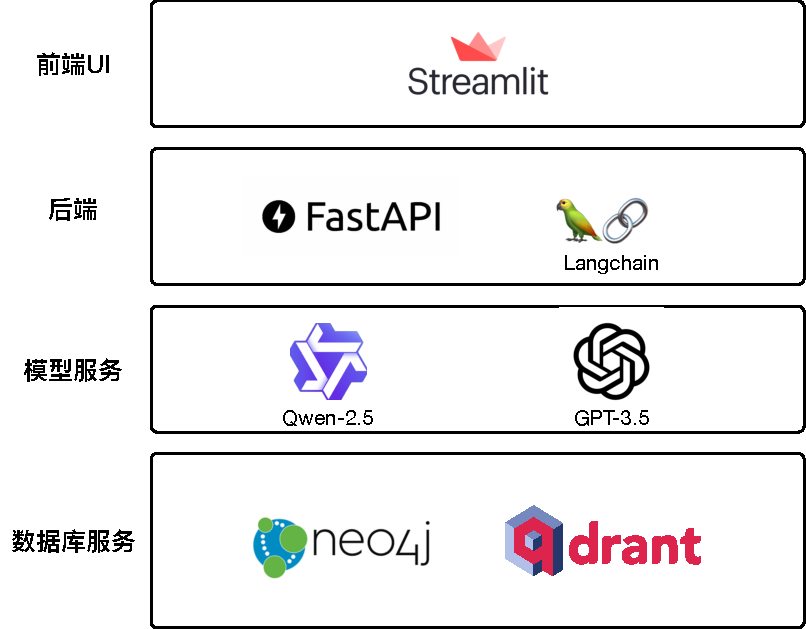
\includegraphics[height=6cm]{../assets/ch5-系统实现图.pdf}
  \bicaption{系统技术实现图}{System Technical Implementation Diagram}
  \label{fig:ch6-implementation}
\end{figure}

在本地大语言模型部署时,我们选择vLLM来部署Qwen模型,vLLM能提供业内顶尖的推理效率、高效的注意力管理机制和对模型量化的支持,还能够将模型部署为OpenAI API格式,提供了方便的交互。
在调用GPT-4o模型时,我们使用的是通过API进行调用。
对于大语言模型智能体搭建过程,我们使用的是LangChain大语言模型框架,该框架能够支持
高效的提示词配置和上下文管理等功能,因此我们的所有大语言模型智能体都通过该框架来搭建。
由于本系统搭建了多个智能体,涉及到智能体之间的合作,我们引入了 LangGraph 来管理大语言模型智能体之间的输入输出工作流。该方法有效提升了系统的鲁棒性,同时优化了代码结构和可维护性。
我们在该系统采用了前后端分离的方式,选择了FastAPI作为后端框架,将除模型推理服务外的服务都以API接口的形式提供,前后端通过HTTP进行通讯。
在前端页面部分,我们选用了目前大语言模型有关应用有关最流行的前端框架之一———Streamlit前端框架来实现。

下面我们将会根据一个具体的使用样例,对该系统的主要页面进行展示。

图\ref{fig:ch6-login}展示了本系统的登录页面,用户通过输入用户名和密码通过系统的鉴权,从而跳转到系统的
功能访问页面。

\begin{figure}[H]
  \vspace{1em}
  \centering
  \setlength{\abovecaptionskip}{10pt} % 控制图片和caption之间的距离
  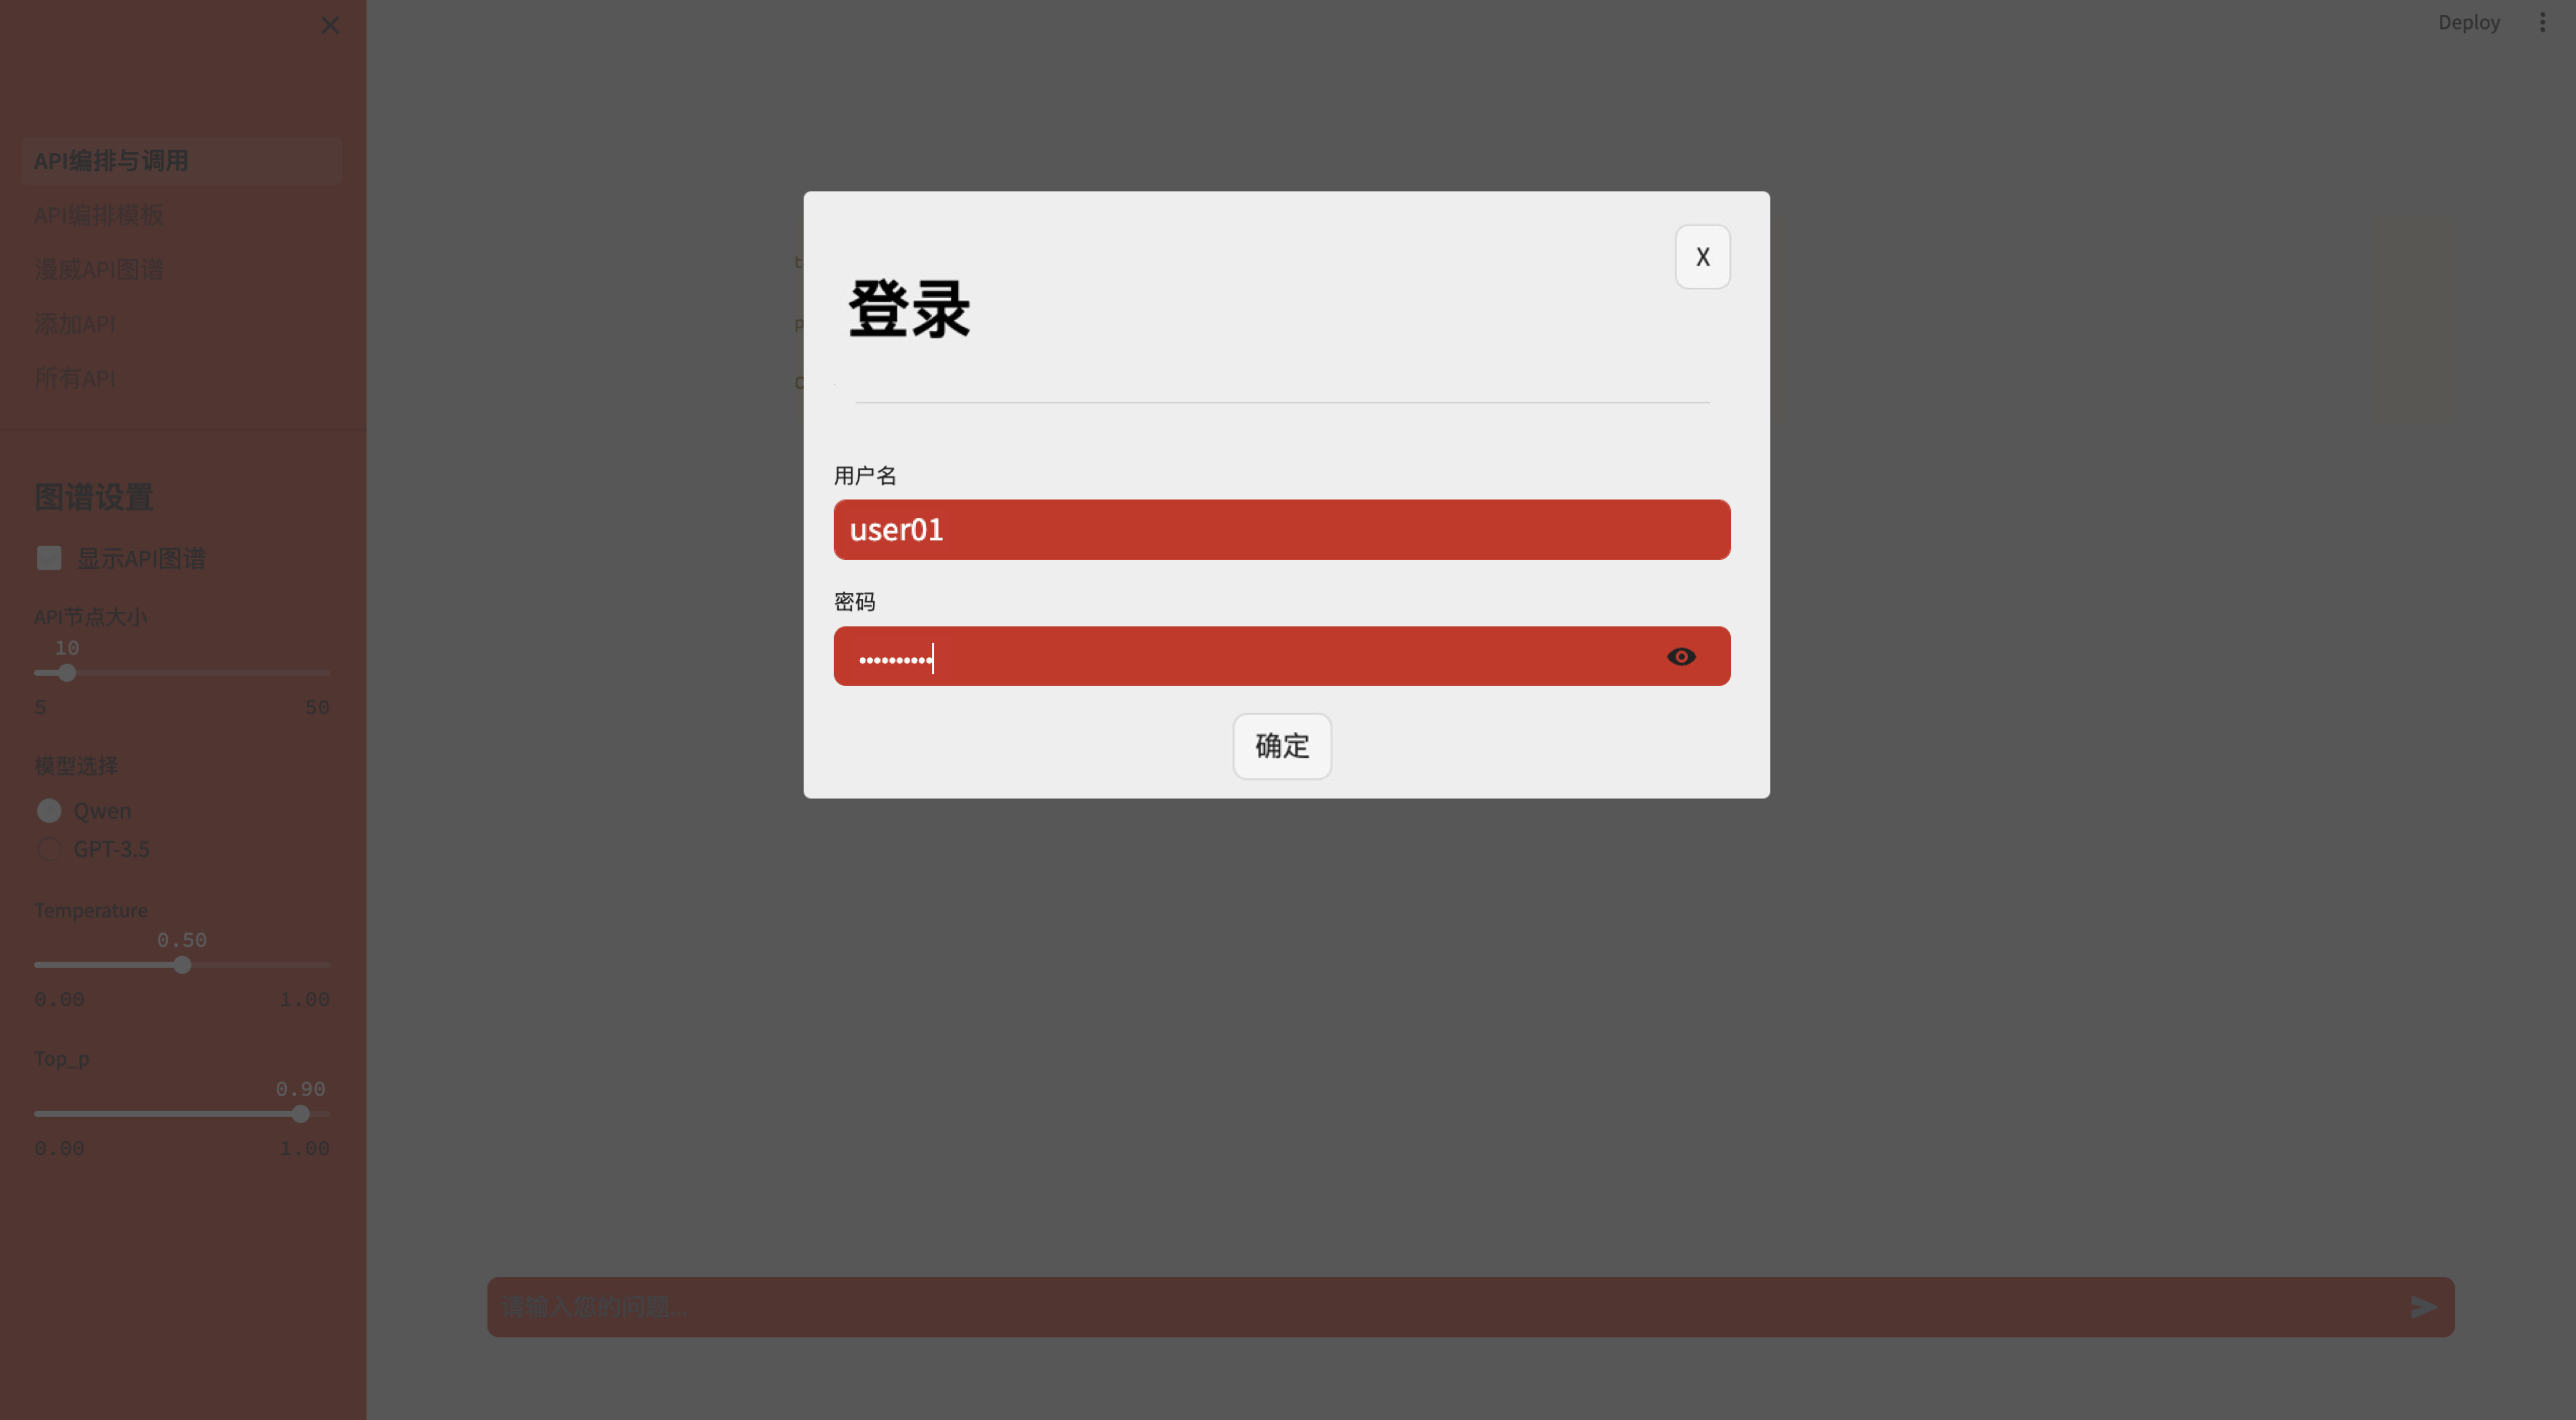
\includegraphics[height=8cm]{../assets/ch6-1登陆.png}
  \bicaption{系统登录页}{System Login Page}
  \label{fig:ch6-login}
\end{figure}

图\ref{fig:ch6-simple-question}展示了本系统的简单问答和工具调用功能。用户通过
页面下方的输入框,通过自然语言的形式描述自己的需求。
系统的输出分为两部分,一部分是自然语言格式的回复,另一部分是
有关工具调用的依赖关系图,作为系统生成对应工具调用路径的依据。
同时,为了提供良好的即使交互体验,本系统采用流式输出的方式展示模型输出的结果,允许用户看到模型的生成过程,减少用户等待,提升用户体验。

\begin{figure}[H]
  \vspace{1em}
  \centering
  \setlength{\abovecaptionskip}{10pt} % 控制图片和caption之间的距离
  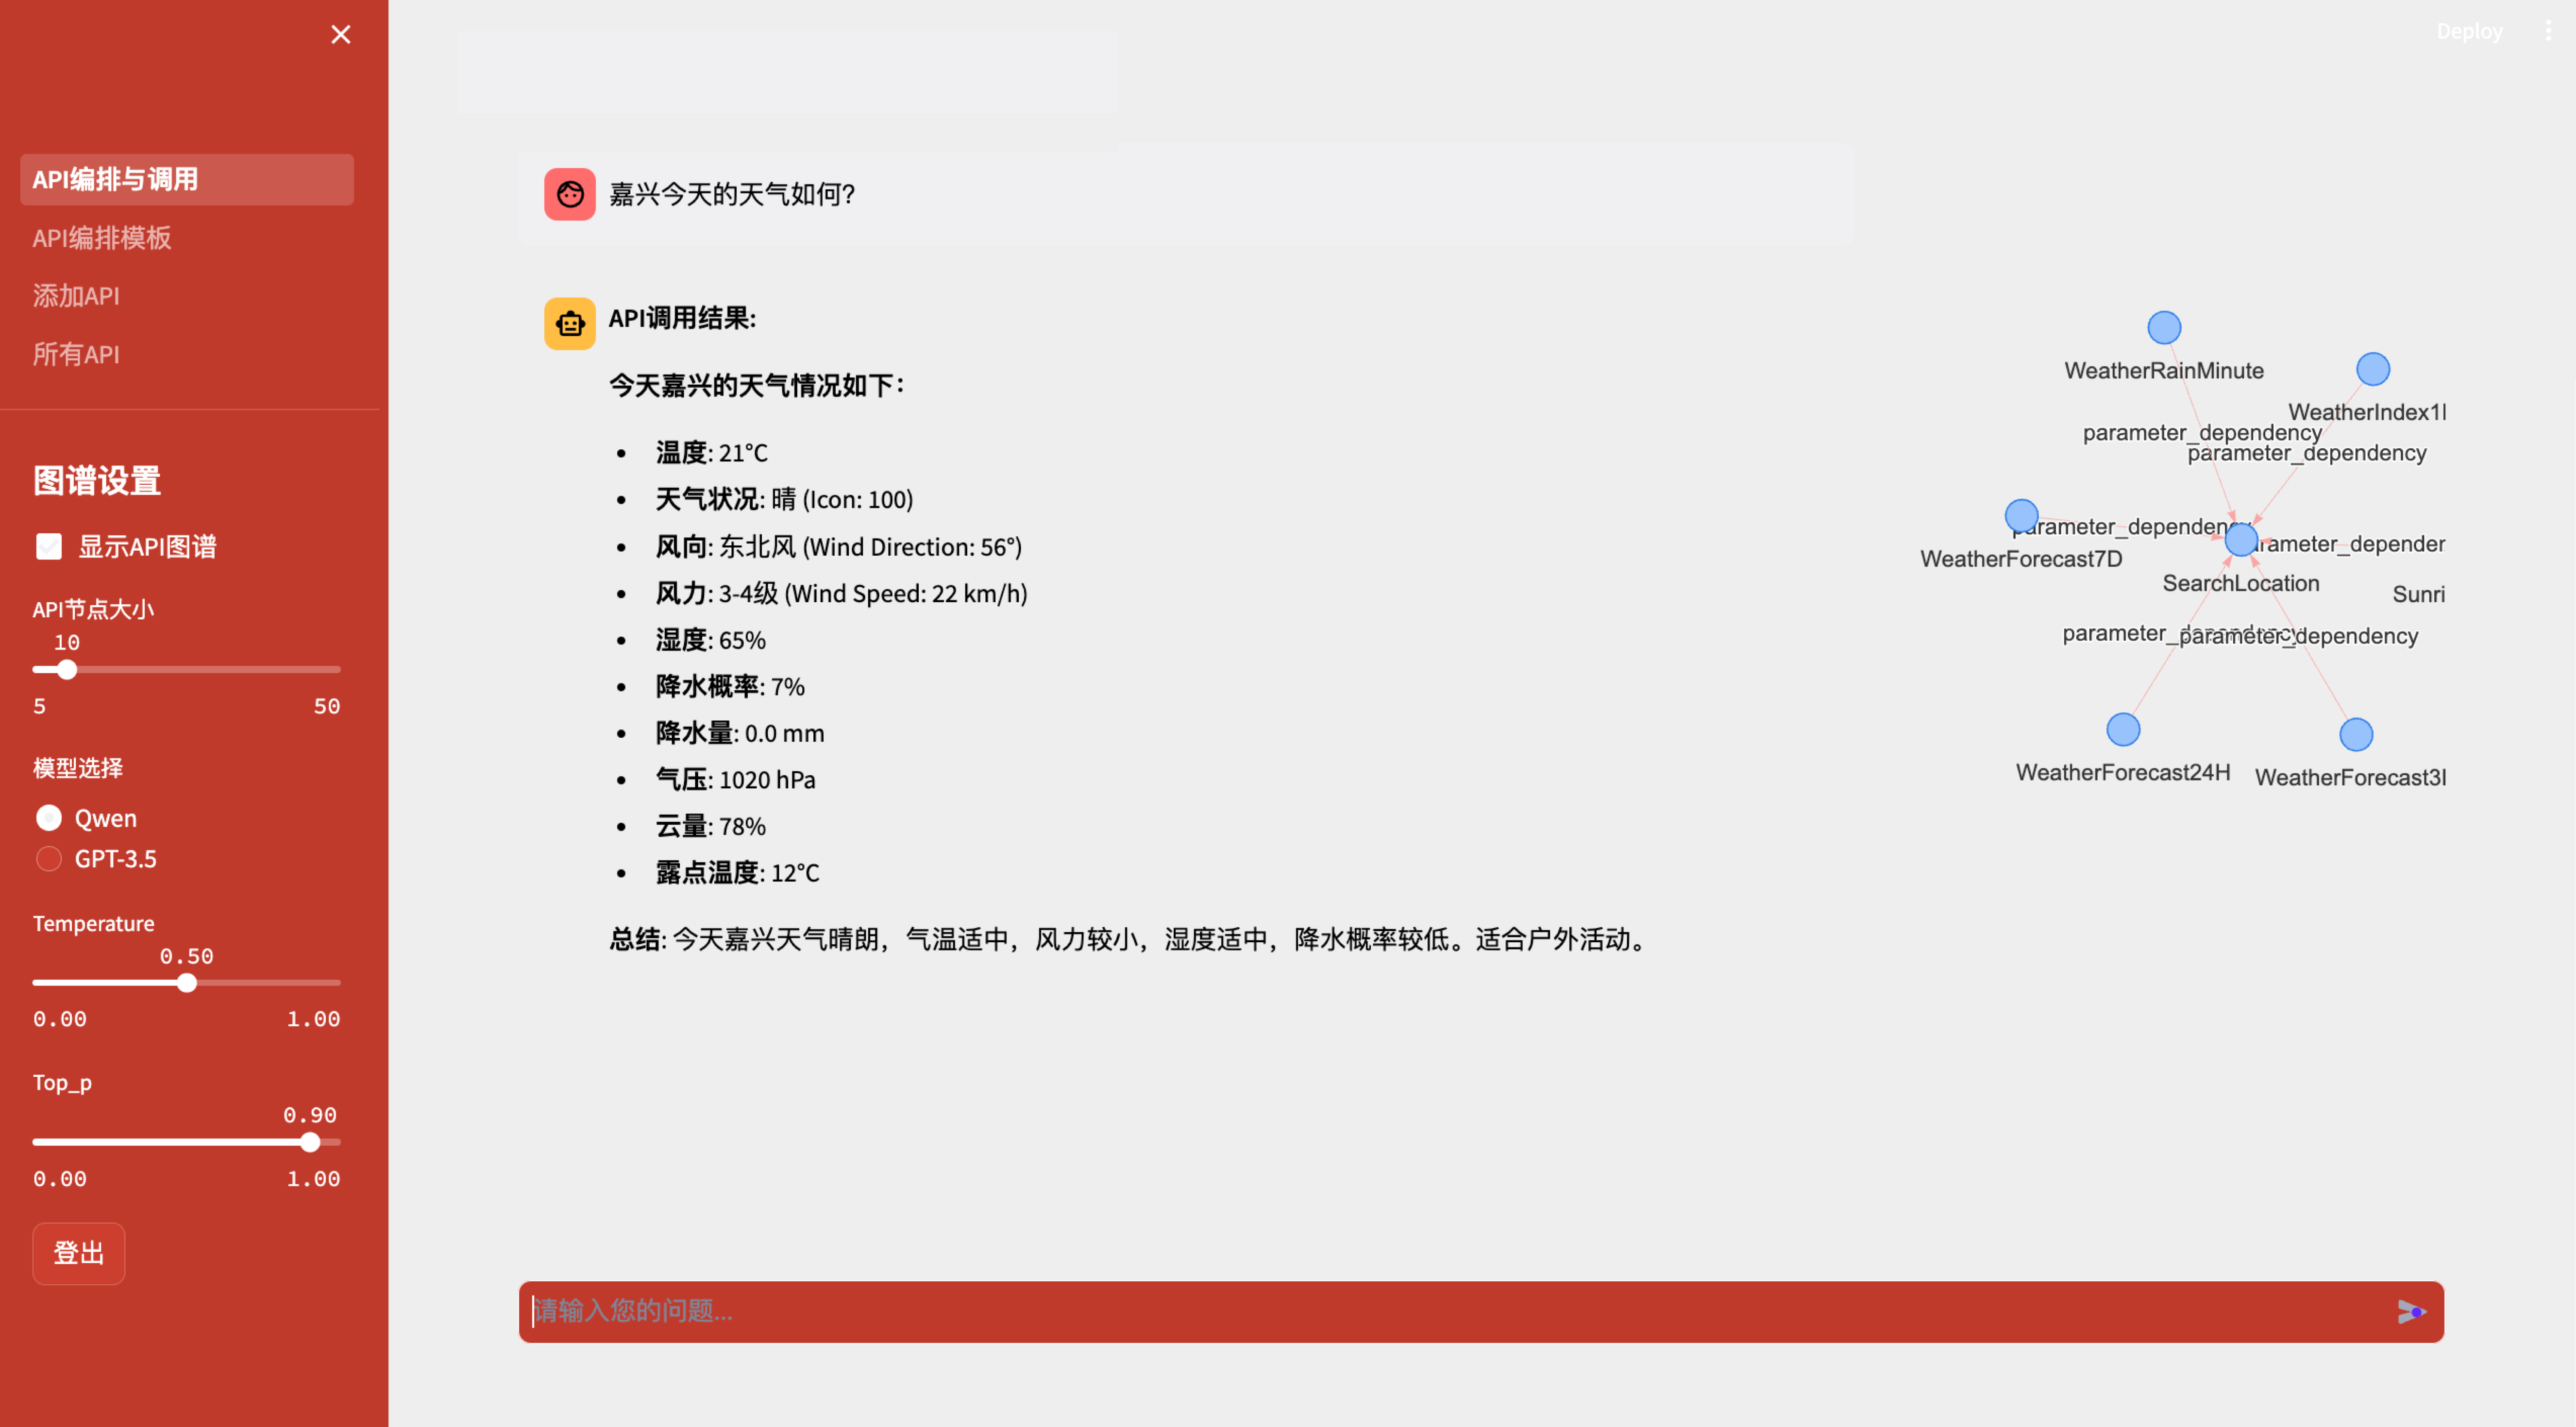
\includegraphics[height=8cm]{../assets/ch6-2简单问题回答.png}
  \bicaption{系统智能问答页}{System Response Page}
  \label{fig:ch6-simple-question}
\end{figure}

图\ref{fig:ch6-all-tools}展示了本系统的工具浏览页,本系统维护的所有工具都会
展示在该页面,包括其名称、工具描述、输入参数、工具类别等。用户或管理员可以浏览该工具信息页来了解本系统集成的工具类型。

\begin{figure}[H]
  \vspace{1em}
  \centering
  \setlength{\abovecaptionskip}{10pt} % 控制图片和caption之间的距离
  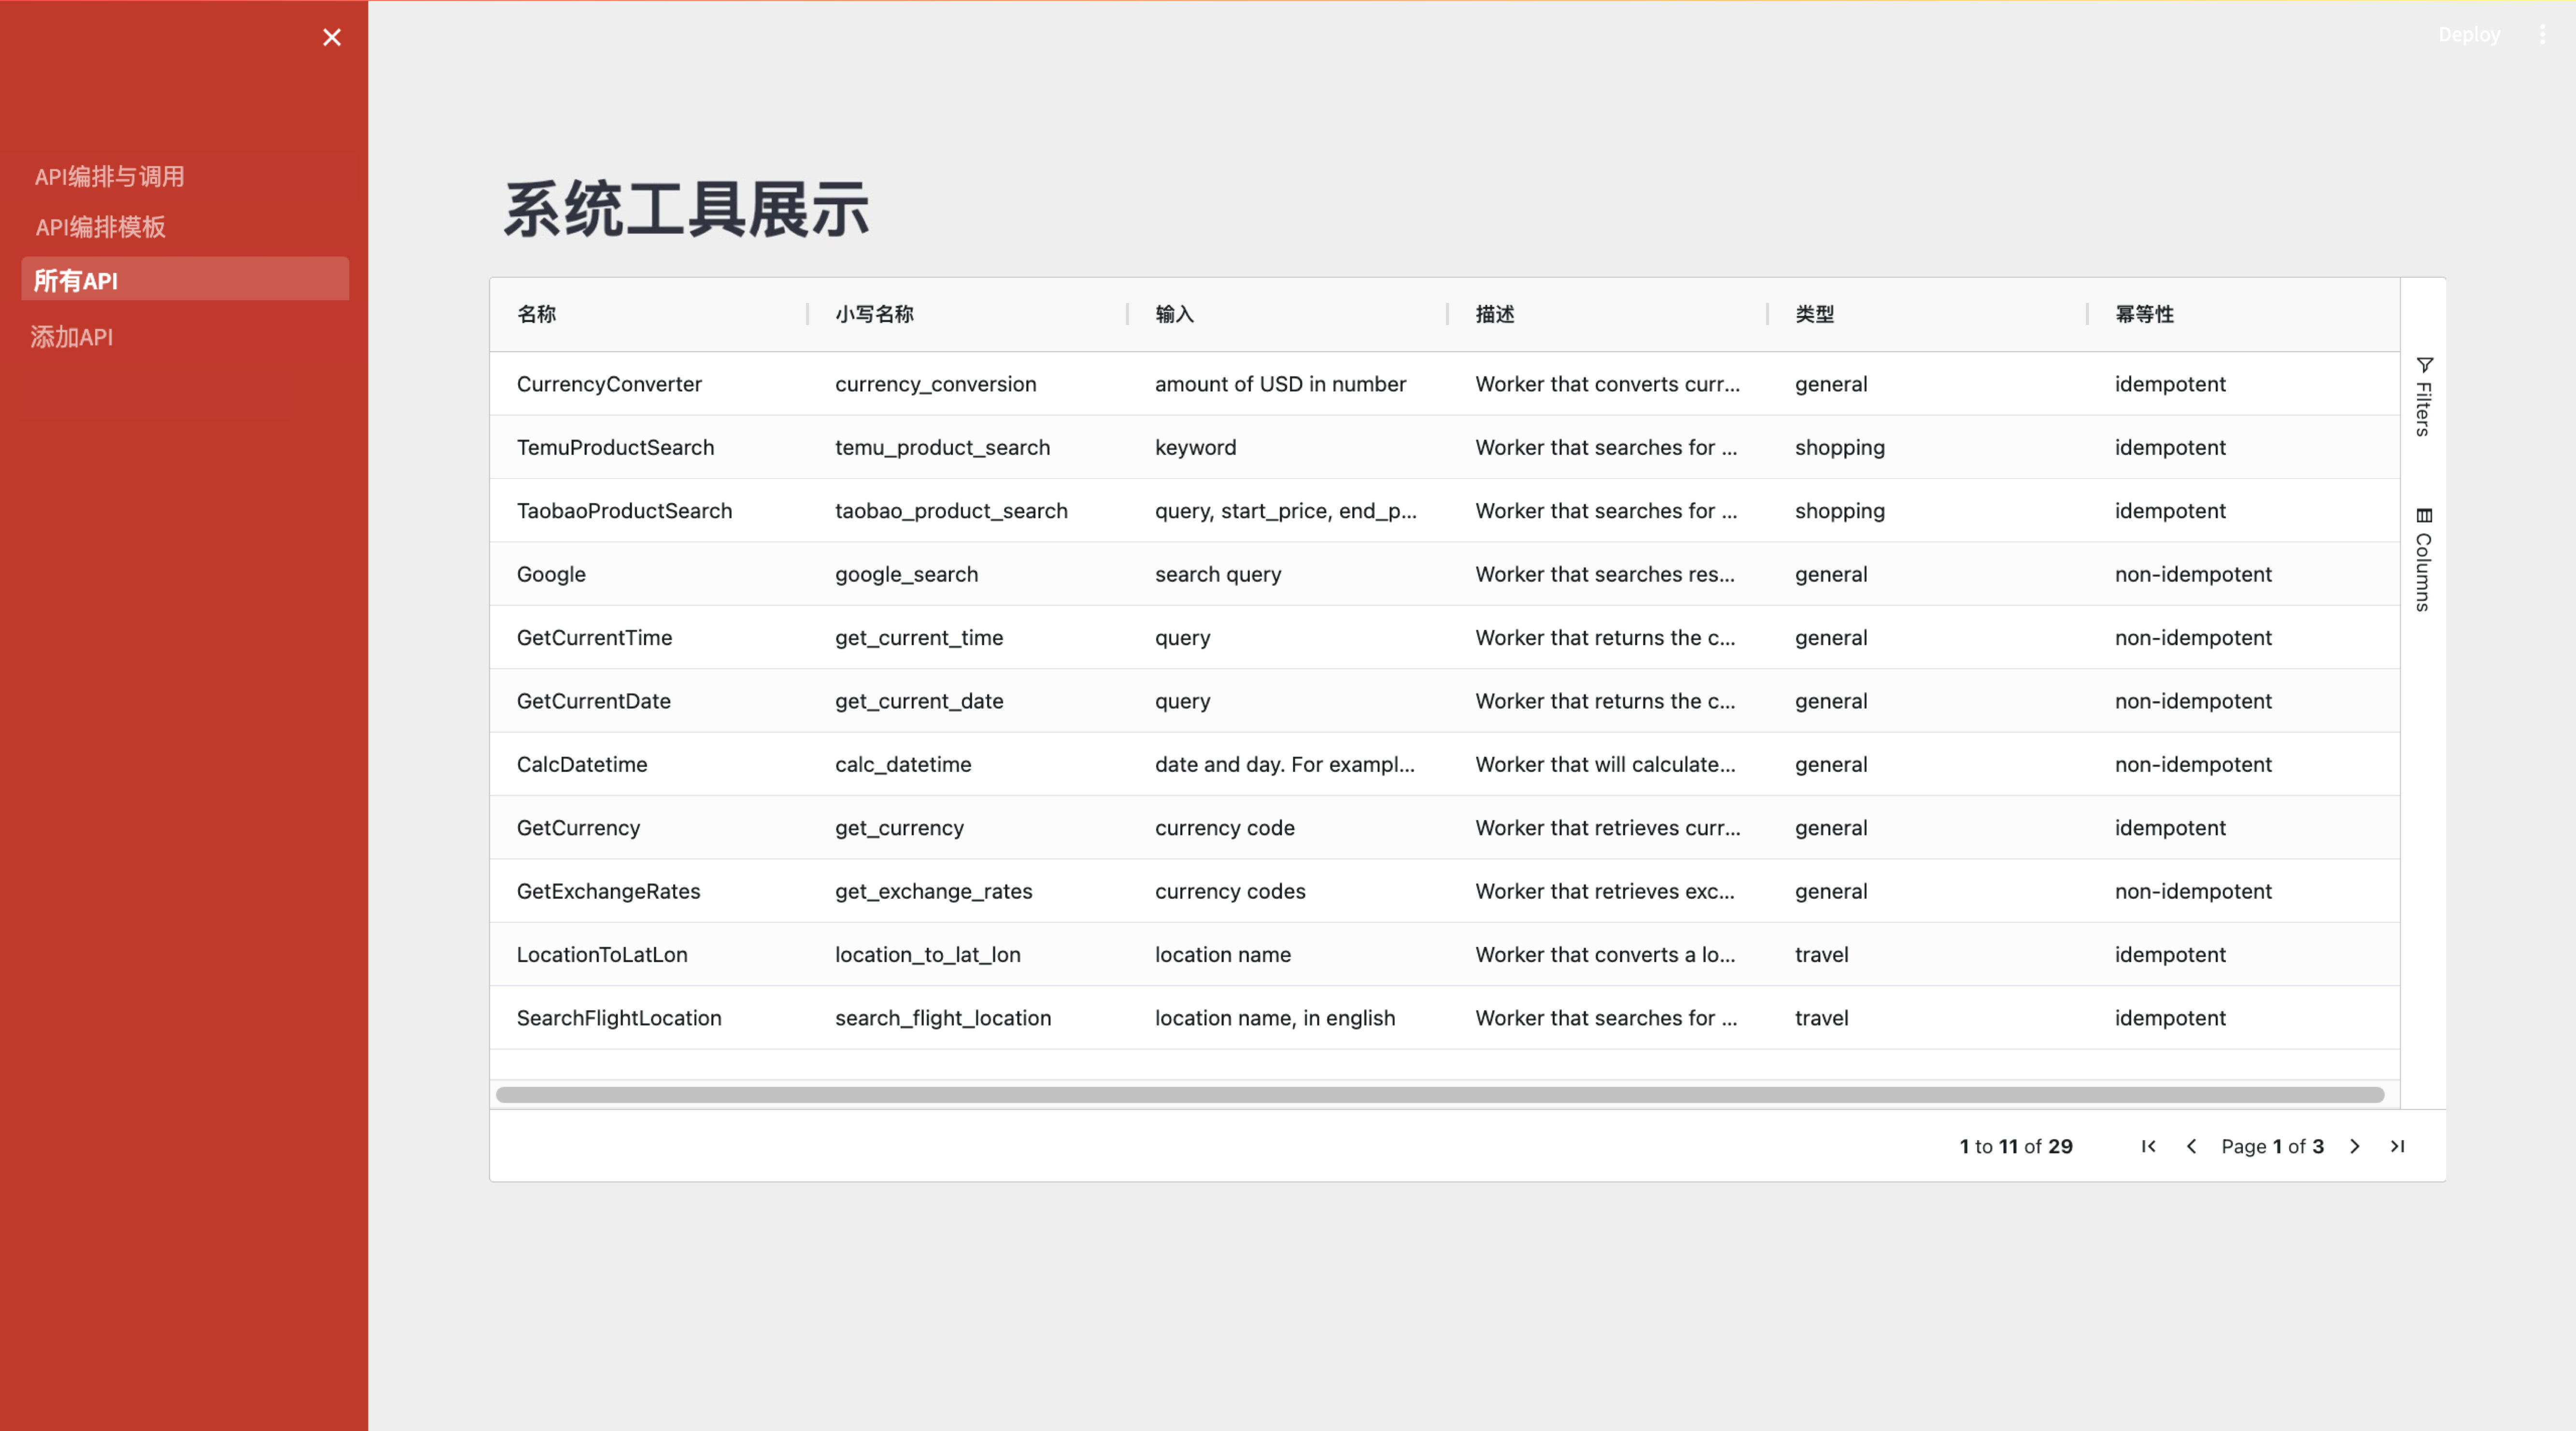
\includegraphics[height=8cm]{../assets/ch6-所有API展示.png}
  \bicaption{工具信息浏览页}{Tools Display Page}
  \label{fig:ch6-all-tools}
\end{figure}

图\ref{fig:ch6-tool-kg} 展示了本系统的工具图谱可视化页面,它与上方的工具浏览页形成了互补的关系。在工具浏览页中,用户可以查看各个工具的详细信息,但无法直观了解工具之间的关联。而在工具图谱可视化页面中,用户可以显式地看到工具之间的参数依赖关系和时序依赖关系,补充了工具浏览页的信息空白。
我们对图谱中的工具组和工具节点进行了颜色上的区分,使用户能够辨别工具组与工具之间的从属关系。

\begin{figure}[H]
  \vspace{1em}
  \centering
  \setlength{\abovecaptionskip}{10pt} % 控制图片和caption之间的距离
  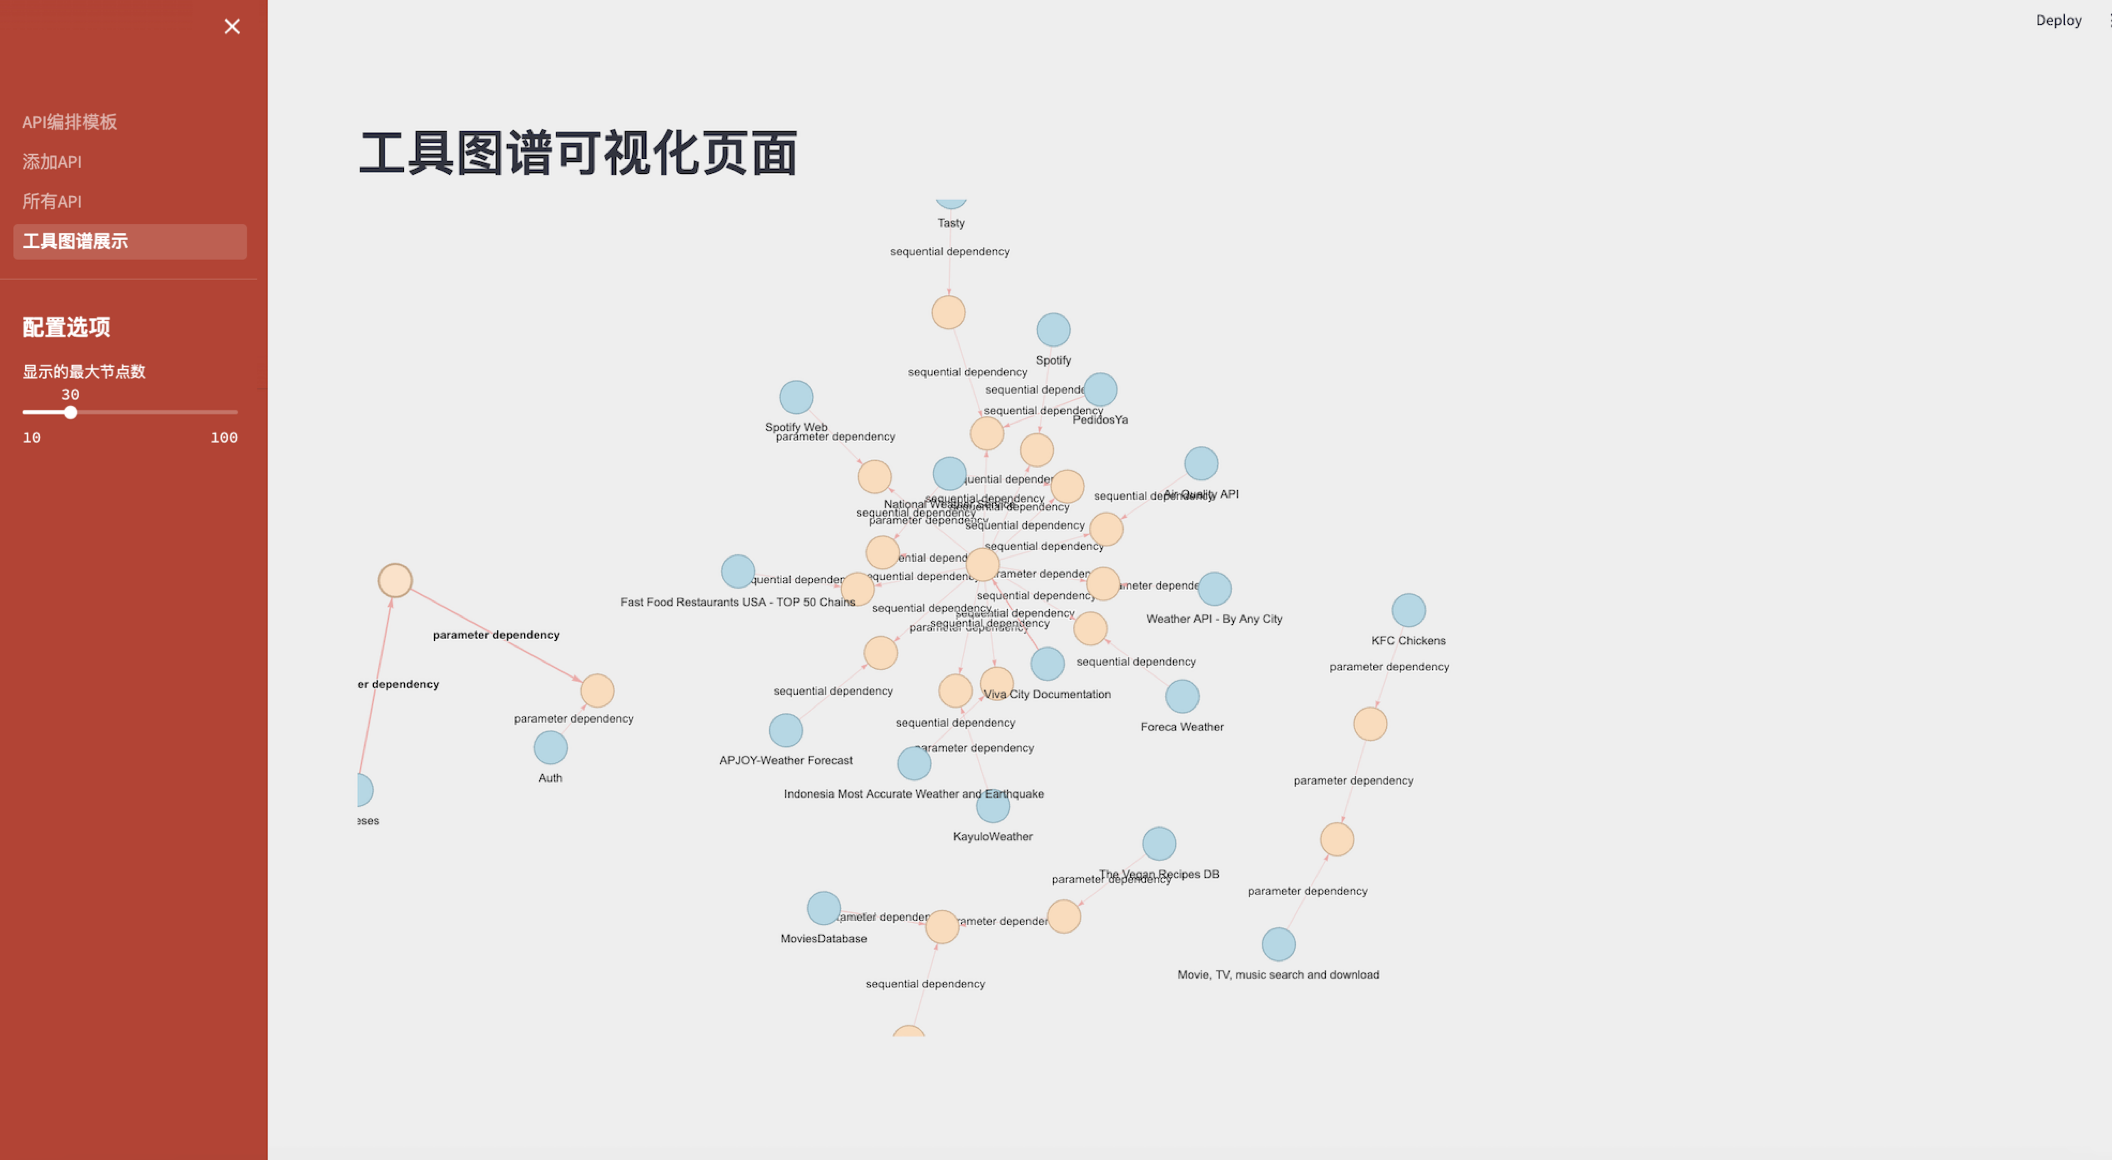
\includegraphics[height=8cm]{../assets/ch6-工具图谱可视化.png}
  \bicaption{工具知识图谱可视化页}{Tool Graph Visualization Page}
  \label{fig:ch6-tool-kg}
\end{figure}

图\ref{fig:ch6-add-tool}展示了本系统的自定义工具添加页面。用户通过填写工具相关的必要信息(如API名称、工具组、请求地址及参数等),即可将自定义API导入系统。此外,页面提供的测试功能支持用户在添加前验证API的可用性。为提升系统的稳定性并确保用户配置的正确性,仅当测试返回码为200时,工具才可成功添加至系统。

\begin{figure}[H]
  \vspace{1em}
  \centering
  \setlength{\abovecaptionskip}{10pt} % 控制图片和caption之间的距离
  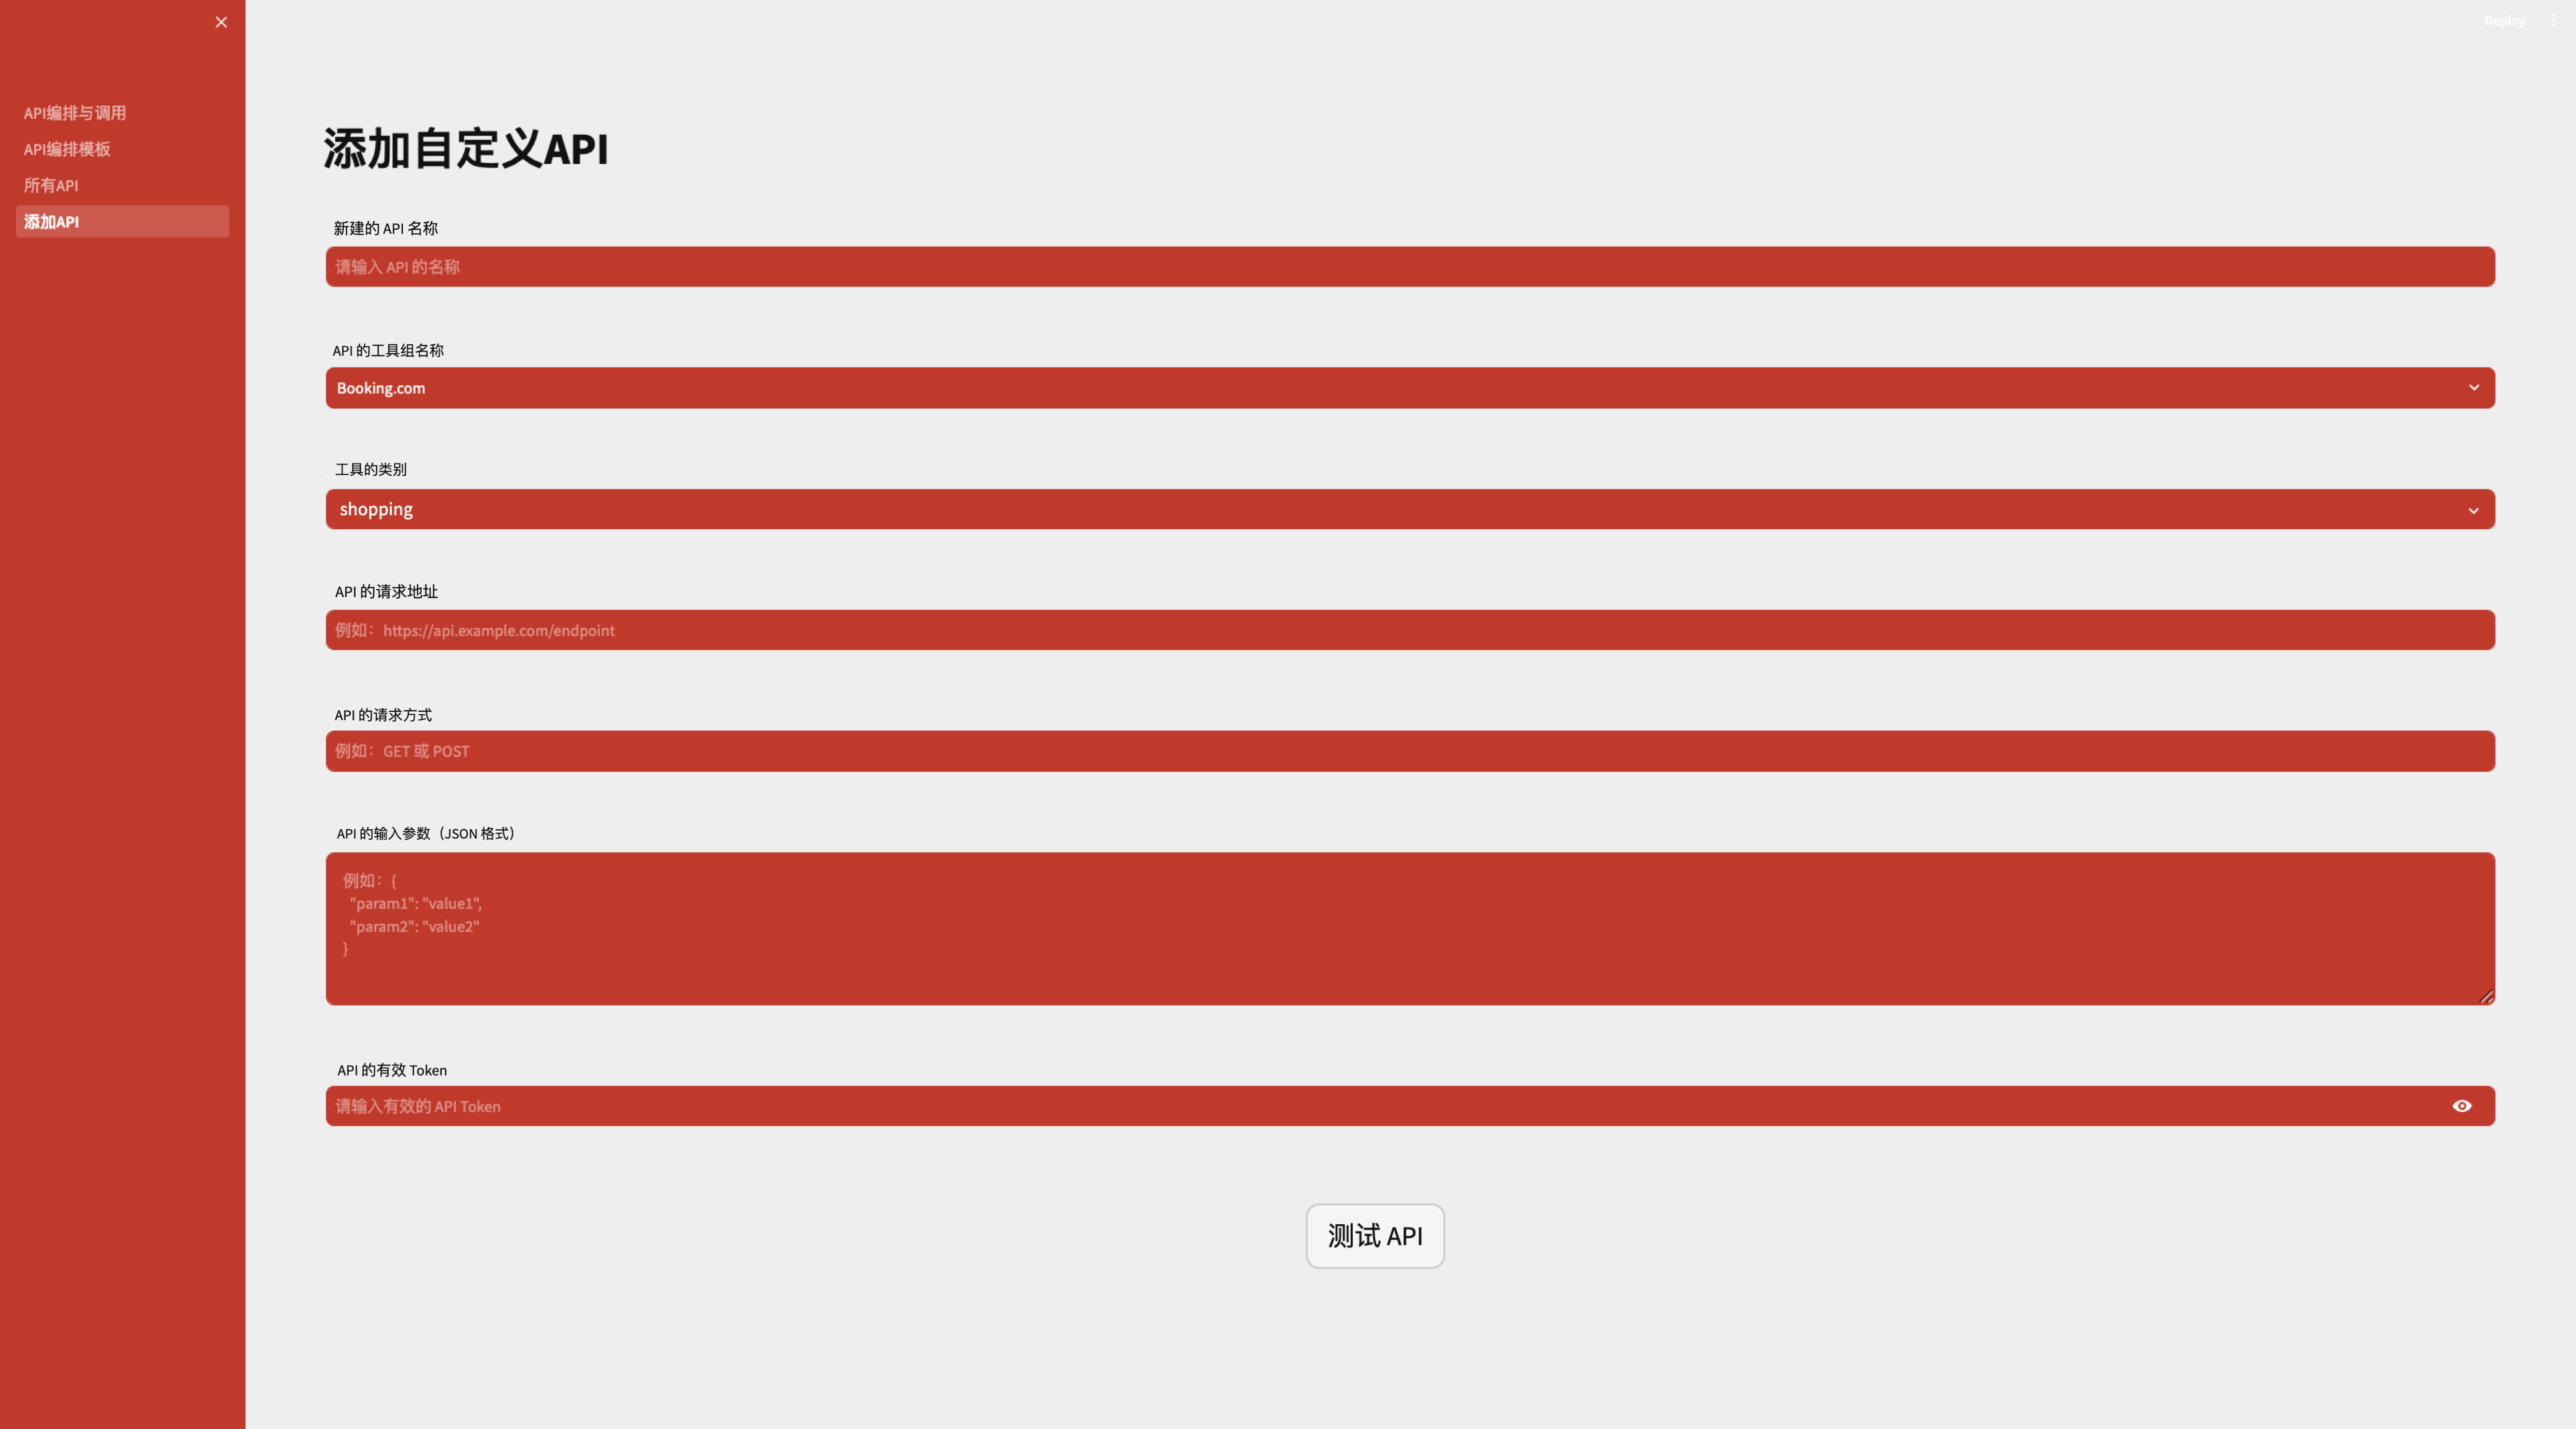
\includegraphics[height=8cm]{../assets/ch6-添加自定义API.png}
  \bicaption{添加自定义API页}{Add Tool Page}
  \label{fig:ch6-add-tool}
\end{figure}

\section{本章小结}

本章设计并实现了一个基于知识图谱和大语言模型智能体机制的API编排与调用系统。系统通过集成知识图谱查询、模型管理和向量相似度计算功能,为用户提供自然语言交互的低门槛界面,并支持复杂需求的API调用和回答生成。系统架构分为存储层、访问层、功能层、接口层和展示层,涵盖从数据存储与检索到用户交互的全链路设计。主要功能包括任务分解模块与API动态编排、API调用流程管理、历史调用参考、自定义工具扩展以及多轮问答支持。系统实现采用FastAPI作为后端框架,结合Streamlit前端和Neo4j、Qdrant等数据库,实现了模块化、用户友好、可扩展的交互体验,满足了多样化的用户需求并提供高效的API编排与调用服务。